\documentclass[conference]{IEEEtran}
\IEEEoverridecommandlockouts

% Packages
\usepackage{cite}
\usepackage{subcaption}
\usepackage{amsmath,amsfonts}
\usepackage{algorithm}
\usepackage{algpseudocode}
\usepackage{graphicx}
\usepackage{textcomp}
\usepackage{xcolor}
\usepackage{booktabs}
\usepackage{adjustbox}
\usepackage{listings}
\usepackage{hyperref}
\usepackage{verbatim}
\usepackage{multirow}
\usepackage{placeins}

\newcommand{\todo}[1]{\color{red} TODO #1 \color{black}}
\newcommand{\torem}[1]{\color{olive} #1 \color{black}}

\def\BibTeX{{\rm B\kern-.05em{\sc i\kern-.025em b}\kern-.08em
    T\kern-.1667em\lower.7ex\hbox{E}\kern-.125emX}}



\begin{document}

\title{Deliverable report \\
\footnotesize \textit{"Matteo Di Noia": Mat: 258426, \texttt{matteo.dinoia@unitn.it}, GitRepo: \texttt{\href{https://github.com/matteo-dinoia/GPU-Computing-2025-258426}{matteo.dinoia/GPU-Computing-2025-258426}}}}

\maketitle

\begin{abstract}
%\torem{[max 200 words]}\\
The sparse matrix-dense vector multiplication (SpMV) is a common linear algebra operation involving a sparse matrix and a dense vector. SpMV is widely used in many real-world applications such as scientific computing and graph analytics.

This deliverable covers one of the possible representation used for sparse matrix in SpMV, COO. It also only discuss GPU implementation without shared memory usage, using only primitive synchronization and the CPU implementation. Finally it discusses what are the limiting factors of COO.
\end{abstract}

\begin{IEEEkeywords}
Sparse Matrix, SpMV, CUDA, Parallelization, Storage Format
\end{IEEEkeywords}

\section{Introduction}
%\torem{[max 300 words]Introduce SpMV application and its parallelization challenges \dots}\\

Sparse matrix vector multiplication (SpMV) is a core computation that is at the foundation of every implicit sparse linear algebra solver. It is also one of the most common primitive in scientific computing, and graph analytics, eg. it is present in software such as MatLab and Numpy.

Due to being an intrinsically memory-bound algorithm, its performance are limited by the memory bandwidth between the process and the memory, especially on highly parallelized, throughput-oriented architectures such as GPU.


\section{Problem Statement}
%\torem{Define the problem statement, including a description of the storage format used and a brief discussion of the parallelization approach (e.g., using CUDA).}
Sparse matrix vector multiplication (SpMV) is defined as the matrix multiplication between a sparse matrix $A$ of size $n\times m$ and a dense vector $x$ of size $m\times 1$ which result in a vector $y$ of size $n\times 1$ computed as follows:
\[y=A \cdot x\]
\[y_i = \sum_{k=1}^{n}A_{ik} x_{k}\]

An efficient implementation of SpMV present various challenges, most of which are related to the storage format and memory access. As said before SpMV is memory-bound and as such an efficient memory access is required to reduce the memory bottleneck. In fact the arithmetic intensity of the worst case of SpMV is very low:
\[Intensity = \frac{2\ flop}{6 \cdot 4\ bytes} = 0.083\frac {flop}{bytes}\]

In order to have a efficient access to the memory a storage format that facilitate such access is required.

\subsection{Storage Format}
%\torem{Details about the format (e.g., CSR, COO, etc.) \dots}

Multiple format exists such as Compressed Sparse Row (CSR), Coordinate (COO), ELLPACK (ELL), etc. In the present paper, the analysis is concentrated on the COO format. The latter is the simplest one in which three array are used:

\begin{itemize}
	\item \textbf{rows (/Ys)}: representing for every $i$ the row (or $y$ value), in which the $i$-th element of the matrix is;
	\item \textbf{cols (/Xs)}: representing for every $i$ the column (or $x$ value), in which the $i$-th element of the matrix is
	\item \textbf{values}: representing for every $i$ the value of $i$-th element;
\end{itemize}

Instead the CSR format, which is explained here to understand the limiting factors of COO, is still composed of the same three array but the rows array is compressed as the name implies. The compressed rows array contains pointers that mark the beginning of rows within the column array. This compression can be achieved by the fact that the points in the three array are assumed to be sorted by row index.

\subsection{Parallelization}
%Describe the CUDA implementation approach \dots
Being SpMV a conceptually easy operation, the simplest way to parallelize it is to exploit independence between operation on some blocks of data, to obtain data parallelism. In the case of SpMV, the way to do it is to execute the computation of each matrix's row concurrently. This is possible because to compute the product of a row and the vector it is only needed read access to the previous two and write access to a single element of the result vector which is independent to the other elements in the same vector, so there is no write conflict and as such no synchronization primitive are required to preserve correctness of the algorithm. This idea can be implemented in CSR as we can get the start of each row.

In COO instead this is not easily possible. To achieve this result we either have to convert the matrix to CSR  or we can find at runtime the start of each row and only after execute thread/s for each row. Both require something similar to a conversion to CSR defeating the purpose of storing the matrix as COO instead of CSR, and the latter massively increase the time as that is not an easily parallelized operation and require to scan the entirety of the Ys array before computing the SpMV.

For this reason we avoid this strategy and instead focus on the use of atomic operation to maintain correctness, in particular, with the use of $atomicAdd$.

\section{State of the Art}
The state of art SpMV for CPU is OpenBLAS, which is an optimized BLAS (Basic Linear Algebra Subprograms). On the other hand, cuSPARSE is a Cuda based GPU accelerated BLAS which perform significantly faster than CPU only alternatives thanks to the higher degree of parallelization. Both of this API are massively more efficient than the algorithm presented here.

\section{Methodology and Contributions}\label{sec:methodology}

%escribe the methodology used during the analysis, the compared algorithms and the expected outcomes. Use pseudo-codes like Algorithm \ref{alg:COOaggr} to describe your own implemented kernels.

%\noindent Include at least the following implementations:
%\begin{itemize}
%    \item Naive CPU implementation
%    \item Optimised CPU implementation based on cache behaviour
%    \item GPU naive implementation
%\end{itemize}

For the analysis, a COO \ref{alg:COO_CPU} and CSR \ref{alg:CSR_CPU} naive CPU implementations were created. Both access data in the sparse matrix $A$ sequentially and the resulting vector $Y$ partially sequentially, sacrificing instead the sequentiality in the access of the dense vector $v$.

Because of the size difference between CSR and COO, with CSR being smaller because of the compressed rows array, we expect the throughput of the latter to be greater than the one of COO as both are memory-bound application.

\begin{algorithm}[h!]
	\caption{COO SpMV on CPU}
	\algorithmicrequire~The input vectors $Ar$, $Ay$, $Av$ representing the COO matrix of size $nnz$, the vector $X$ of size $nrows$.
	\begin{algorithmic}[1]
		\Procedure{Function}{$Ar$, $Ay$, $Av$, $X$, $nnz$}
		\For{$k$ in $\{1 \dots nnz\}$}
		\State $Y[Ay[k]] = Y[Ay[k]] + Av[k] * X[Ax[k]] $\label{partitioning}
		\EndFor
		\State \textbf{return} $Y$\Comment{the result vector}
		\EndProcedure
	\end{algorithmic}
	\label{alg:COO_CPU}
\end{algorithm}

\begin{algorithm}[h!]
	\caption{CSR SpMV on CPU}
	\algorithmicrequire~The input vectors $Ar$, $Acy$, $Av$ representing the CSR matrix of size $nnz$, the vector $X$ of size $nrows$.
	\begin{algorithmic}[1]
		\State $k \leftarrow 0$
		\Procedure{Function}{$Ar$, $Acy$, $Av$, $X$, $nnz$, $nrows$}
		\For{$r$ in $\{1 \dots nrows\}$}
		\State $end \leftarrow Acy[r + 1]$
		\While{$k < end$}
		\State $Y[r] \leftarrow Y[r] + Av[k] * X[Ax[k]] $\label{partitioning}
		\State $k \leftarrow k + 1$
		\EndWhile
		\EndFor
		\State \textbf{return} $Y$\Comment{the result vector}
		\EndProcedure
	\end{algorithmic}
	\label{alg:CSR_CPU}
\end{algorithm}

After this it is possible to expand the COO implementation by simply parallelize the for and replacing the additions with a $atomicAdd$ \ref{alg:COO_GPU} .

\begin{algorithm}[h!]
	\caption{COO SpMV on CPU}\textsc{}
	\algorithmicrequire~The input vectors $Ar$, $Ay$, $Av$ representing the COO matrix of size $nnz$, the vector $X$ of size $nrows$.
	\begin{algorithmic}[1]
		\Procedure{Function}{$Ar$, $Ay$, $Av$, $X$, $nnz$}
		\For{$k$ in $\{1 \dots nnz\}\ \textbf{parallel}$}
		\State $atomicAdd(Y[Ay[k]],\ Av[k] * X[Ax[k]]) $\label{partitioning}
		\EndFor
		\State \textbf{return} $Y$\Comment{the result vector}
		\EndProcedure
	\end{algorithmic}
	\label{alg:COO_GPU}
\end{algorithm}

But this simplicity comes with a cost: performance. In fact, atomic operation are never cheap and as such it is expected that this algorithm will not even be close to the theoretical worst-case, instead it will be much worse.

But, there are some possible change that can be done to reduce cache missed and improved performance, as detailed in the following chapters.

\section{System Description and Experimental Set-up}
%Use this section to describe system, dataset and experimental set-up.

\subsection{System Description}
%Describe the used system and the software environment (CUDA version, GCC version, \dots). Decide which information are valuable to group into a table like Table \ref{tab:system_description} and which are more valuable to be described in the text.
The previous algorithms were tested with GCC 12.3, CUDA version 12.5 on the $Baldo$ cluster in the partition $edu-short$ only on the node $edu01$. That means the program were run on a system with a "AMD EPYC 9334" 32-Core CPU and as a GPU a "NVIDIA A30", the attributes of the latter can be seen in Table \ref{tab:system_description} .

\begin{table}[htb!]
	\centering
	\begin{adjustbox}{width=0.8\columnwidth}
		\begin{tabular}{lc}
			\toprule
			\textbf{Metrics} &  \textbf{Value}  \\
			\midrule
			Peak FP32 Compute &  10 TFlops   \\
			Peak Memory Bandwidth (HBM2) & 933 GBs  \\
			Maximum number of threads per block & 1024 \\
			Warp size & 32 \\
			\bottomrule
		\end{tabular}
	\end{adjustbox}
	\vspace{1em}

	\caption{System details}
	\label{tab:system_description}
\end{table}

\subsection{Dataset description}

%Describe the used dataset and the reasons of your choice. List the used input matrices and all the information that you think are valuable to show (number of non-zero elements, sparsity ratio, \dots); Table \ref{tab:dataset} gives you a possible example.
To test the implementations we use four datasets \ref{tab:dataset} . The largest one \textit{Mawi}, is also the one with some row and cols that are very dense. Of medium size there are Delaunay with radial elements and Circuit5M which is a mixture of the previous two. Finally the smallest is Model7 with somewhat irregular patterns.
\FloatBarrier
\begin{figure}
	\centering
	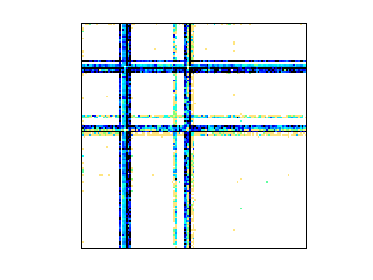
\includegraphics[width=0.3\linewidth]{model_images/mawi_201512020330}
	\label{dat:mawi}
	~
	\includegraphics[width=0.3\linewidth]{model\_images/circuit5M\_dc}
	\label{dat:circuit}

	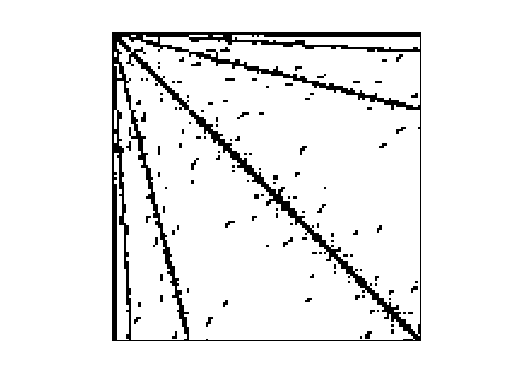
\includegraphics[width=0.3\linewidth]{model_images/delaunay_n23}
	\label{dat:delaunay}
	~
	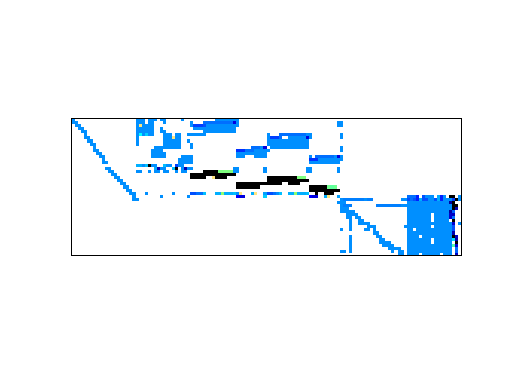
\includegraphics[width=0.3\linewidth]{model_images/model7}
	\label{dat:model7}

	\caption{In the top, the visualization of Mawi and Circuit5c and in the bottom Delaunay and Model7}
	\label{img:data-vis}
\end{figure}

\begin{table}[]
	\centering
	\begin{adjustbox}{width=0.9\columnwidth}
		\begin{tabular}{lrrrrc}
			\toprule
			\textbf{Dataset} & \textbf{Size} & \textbf{Non-zero} \\
			\midrule
			mawi\_201512020330 & 226'196'185$^2$ & 480'047'894\\
			circuit5M\_dc & 3'523'317$^2$ & 14'865'409\\
			delaunay\_n23 & 8'388'608$^2$ & 50'331'568\\
			model7  & 3'358 $\times$ 9'582 & 51'027\\
			\bottomrule
		\end{tabular}
	\end{adjustbox}
	\vspace{1em}

	\caption{Datasets used in the analysis}
	\label{tab:dataset}
\end{table}


\clearpage
\FloatBarrier

\section{Experimental Results}
%Present and discuss results. Include plots and tables when required (like Figure \ref{fig:enter-label}). Do not simply describe the figures; criticise the achieved results by underlining how they confirm/differ from the expected outcomes described in Section \ref{sec:methodology}.

%\noindent For the analysis include
%\begin{itemize}
%	\item Valgrind and runtime comparison between the CPU implementations
%	\item Runtime CPU vs GPU comparison looping over different matrix dimensions
%\end{itemize}
\subsection{CPU implementations}
Using Model7 as datasets to test cache misses, the results are the one in the Table \ref{tab:cache-results} . These values are very rough as cachegrind doesn't allow testing of a single portion of code. As such, both test were conducted in the same exact codebase with the single difference of calling COO or CSR methods (so even the conversion from COO to CSR was done in both).

This minimize the difference between the test but doesn't solve the issue of the initialization causing some misses. To reduce the impact of the initial misses, the SpMV was compute 500 times.

As expected, CSR being compressed cause lower reference and also slightly less cache misses.
\begin{table}[hbt!]
	\centering
	\begin{adjustbox}{width=\columnwidth}
		\begin{tabular}{lrrrrc}
			\toprule
			\textbf{Type} & \textbf{D Refs} & \textbf{D1 misses} & \textbf{LLd misses} & \textbf{D1 miss rate} & \textbf{LLd miss rate} \\
			\midrule
			COO & 429,885,147 & 5,348,505 & 13,417 & 1.2\% & 0.0\% \\
			CSR & 382,093,606 & 4,031,502 & 13,417 & 1.1\% & 0.0\% \\
			\bottomrule
		\end{tabular}
	\end{adjustbox}
	\vspace{1em}

	\caption{Valgrind's cachegrind tool results}
	\label{tab:cache-results}
\end{table}

It was then measured the average time (over 20 cycles with 5 warmup). Time wise instead we see that CSR indeed wins in Model7 and Circuit5c but massively lose in Delaunay and Mawi datasets. In the Table \ref{tab:time-cpu-results} are also reported the bandwidth calculated from the average times, instead of the flops, that is because it is memory bound, so we care more about bandwidth.

\begin{table}[hbt!]
	\centering
	\begin{adjustbox}{width=\columnwidth}
		\begin{tabular}{lcccc}
			\toprule
			\textbf{Datasets} & \textbf{COO avg (ms)} &\textbf{COO (GB/s)} & \textbf{CSR avg (ms)} & \textbf{CSR (GB/s)}\\
			\midrule
			Model7 & 0.118 & 10.32 & 0.111 & 10.992\\
			Delaunay & 77.2 & 7.824 & 126 & 4.8\\
			Circuit5c & 49.8 & 9.252 & 45.4 & 10.152\\
			Mawi & 691 & 8.34 & 976 & 5.892\\
			\bottomrule
		\end{tabular}
	\end{adjustbox}
	\vspace{1em}

	\caption{CPU performance over datasets}
	\label{tab:time-cpu-results}
\end{table}

\FloatBarrier
Unfortunately due to time constraints and technical problem with Valgrind in the cluster, it was not possible to further analyze if these CSR losses are caused by higher cache misses. It may behave been that with larger samples COO will be faster because of higher hit rate.

\subsection{GPU implementations}
The simple idea of a GPU Algorithm \ref{alg:COO_GPU} can be implemented in various ways. The versions tested in this paper are:
\begin{itemize}
	\item \textbf{"Kernel 1 size"}: where each thread acquires locally adjacent elements;
	\item \textbf{"Kernel threads size"}: where the distance between an element and the next that the thread acquire is the \# threads;
	\item \textbf{"Kernel warp size"}: where the distance between an element and the next that the thread acquire is the size of a warp;
	\item \textbf{"Kernel block size"}: where the distance between an element and the next that the thread acquire is the size of a block;
\end{itemize}

It was, then, tested the performance of them, with respect to the number of thread per block and the number of blocks. As expected the first kernel is the worst one and warp size and block size are in the first place, while perform around the same. This is because of the fact that warp share cache and as such threads in same thread should access close position. The reason for "Kernel threads size" to be about half the performance of the warp one it is possibly connected to the fact that each thread need to access location that are pretty far apart, increasing cache misses.

\begin{figure}[hbt!]
	\centering
	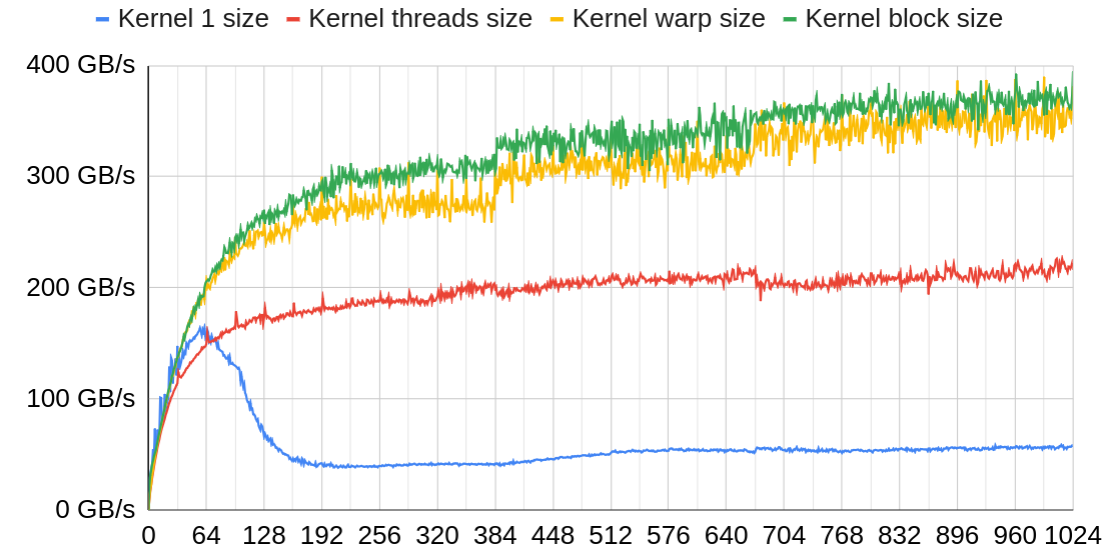
\includegraphics[width=1\linewidth]{data_images/Gb_for_size_block}
	\caption{Throughput over block size of the various kernels }
	\label{fig:gbforsizeblock}
\end{figure}

\begin{figure}[hbt!]
	\centering
	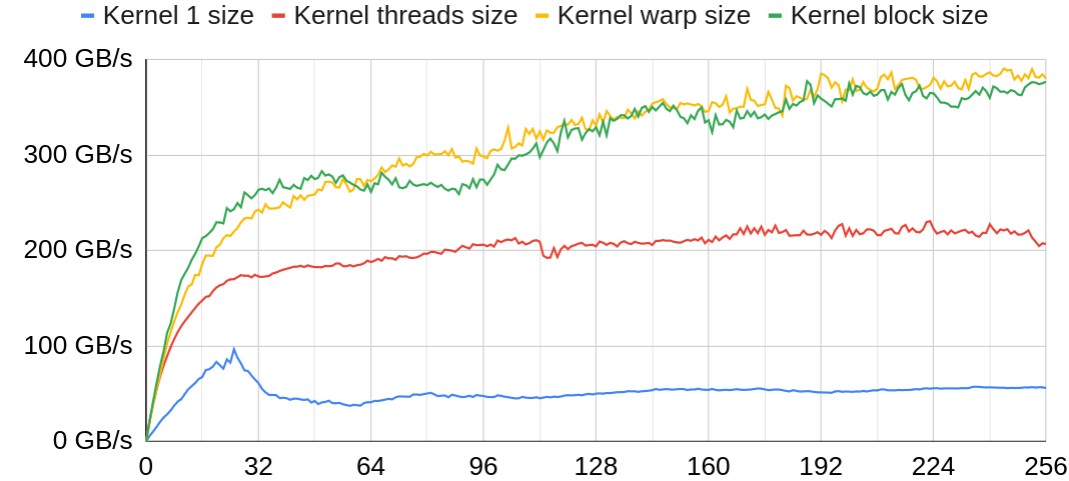
\includegraphics[width=1\linewidth]{data_images/Gb_for_size_grid}
	\caption{Throughput over blocks number of the various kernels}
	\label{fig:gbforsizegrid}
\end{figure}

Also as expected the two graph look very alike. That is because the A30 has only 4 SM with each a warp of size 32, so increasing to values above this value, has similar result if it is done via block size or number of blocks.


\begin{figure}
	\centering
	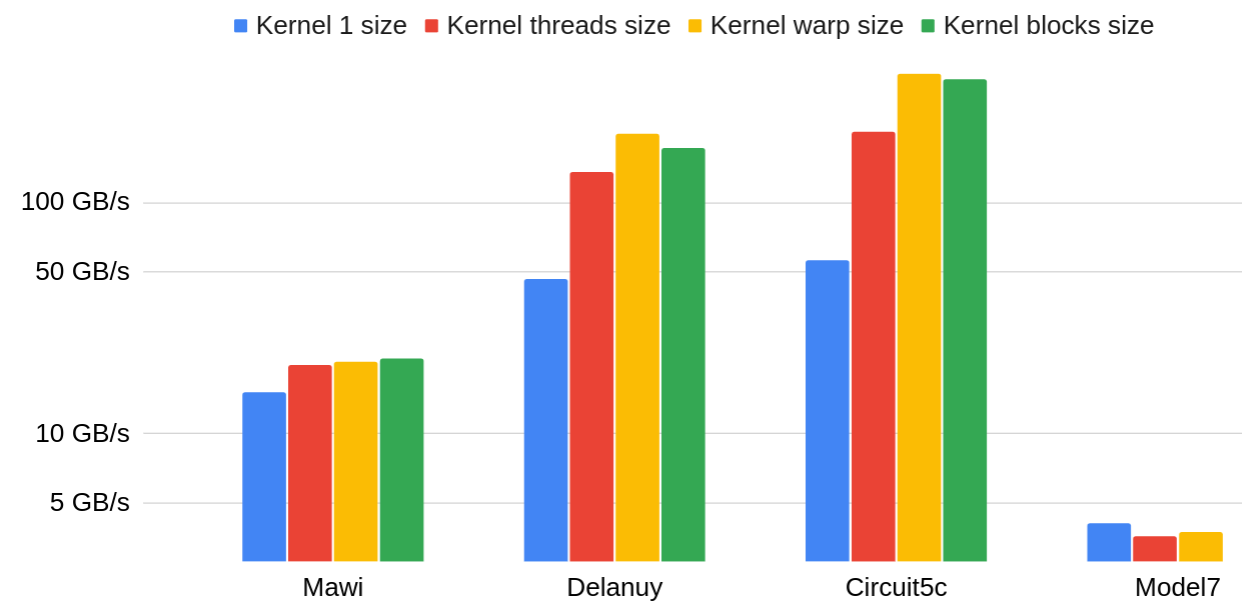
\includegraphics[width=0.9\linewidth]{data_images/perf_gpu}
	\caption{Performance of the kernels based on dataset}
	\label{fig:perf-gpu}
\end{figure}
\FloatBarrier
The kernels were then benchmarked with all the datasets. As it was expected, the worst performance come from the smallest dataset. The cause of this, is that GPU are optimized for throughput and so they have higher latency. So with smaller size datasets the latency become the limiting factor. It can also be noted that on small datasets the comparison between the various kernel become meaningless, as the time is almost all spent on the various overhead (eg. creating a kernel).


\begin{table}[hbt!]
	\centering
	\begin{adjustbox}{width=\columnwidth}
		\begin{tabular}{lcccc}
			\toprule
			\textbf{Kernel} & \textbf{Mawi} & \textbf{Delaunay} & \textbf{Circuit5c} & \textbf{Model7}\\
			\midrule
			Kernel 1 size & 15.1 GB/s & 46.7 GB/s & 56.1 GB/s & 4.08 GB/s\\
			Kernel threads size GB/s & 19.8 GB/s & 136 GB/s & 202 GB/s & 3.6 GB/s\\
			Kernel warp size & 20.5 GB/s & 198 GB/s & 361 GB/s & 3.74 GB/s\\
			Kernel blocks size & 21.1 GB/s & 172 GB/s & 341 GB/s & 2.8 GB/s\\
			\bottomrule
		\end{tabular}
	\end{adjustbox}
	\vspace{1em}

	\caption{Results in table format}
	\label{tab:gpu-results}
\end{table}

\FloatBarrier

Finally we can node how, ignoring Model7, the "Kernel warp size" has the most reliable performance as expected while sometimes the "Kernel block size" has better performance but is not very reliable, having a larger variance.


\section{Conclusions}
In conclusion COO present various problematic aspect when talking about parallelization, requiring atomic operation, in contrast to the CSR implementation. Because of this, the performance obtained are even worse than the theoretical worse case as it was theorized. This can be seen in Image \ref{fig:roofline} .

\begin{figure}[hbt!]
	\centering
	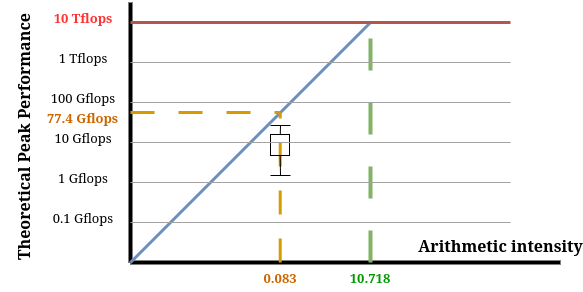
\includegraphics[width=1\linewidth]{data_images/roofline}
	\caption{Roofline model of a NVIDIA A30}
	\label{fig:roofline}
\end{figure}

To be exact the best result obtained is only $37\%$ of the theoretical worst case scenario.
\\

In conclusion, we can assert that COO is not suitable representation for sparse matrix when talking about efficient kernel implementation, especially in the case of a naive implementation. In such cases, it should be instead evaluated the use of CSR.
\end{document}

